%!TEX root = ../thesis.tex

\chapter{模型与实证分析}

\section{理论模型}
\subsection{微观层次}
本文将微观层面影响企业违约的因素分为以下四类,主要包含企业级的指标:
\subsubsection{公司层面}

国企发行了80\%的债券,但违约中只占了15\%,有学者指出可能是由于国企存在政府支持\cite{mo2021china},也有可能国企经营情况较好。因此,本文将公司性质作为影响因素之一建模。

此外,股东对企业的支持也可能影响是否违约,如苏宁易购实控人难以向企业注血,导致苏宁走向违约。
上市企业比非上市企业融资方式更多,融资额通常更大,因此上市与否也可能影响违约。

此外,正如\ref{sec:zs}中对公司治理的研究所揭示,公司治理成效也可能影响违约因素。但是一方面公司治理会影响违约与否,违约企业通常会面临法律纠纷、债权人接管等情况,令企业公司治理发生很大变化。本文计划以持有基金占比作为公司治理的代理变量。公募基金相较于考虑违约与否,更加担心债券持有期间贬值,这就使他们更加担心企业公司治理存在问题,即基金持有比例和公司治理强相关。公募基金持有债券类似于交易性金融资产,而银行持有债券交易更少,类似于持有至到期投资。公募基金在评级下调超出风控阈值后必须斩仓,除非债券流动性过低有价无市,而所有违约债券都会被下调为垃圾级,而评级下调的债券中违约中只是少数,因此公募基金持有比例与违约弱相关。因此本文采用基金持有比例来表征公司治理。

最后,公司层面还有一些难以量化到因素,如发行人主观意愿(花样年地产账面现金充足“花式”躺平违约)、财务造假(康美药业、五洋建设)。但因此违约的是少数,绝大多数地产商苦苦挣扎避免躺平,绝大多数企业报表准确。因此本文不将这些因素纳入考虑。
\subsubsection{经营层面}
企业面临流动性危机,很多情况下是经营不及预期,营收大幅亏损,进而导致违约。

客户集中度过高,可能会导致企业面临较高的风险\cite{王雄元2017客户集中度与公司债二级市场信用利差}。集中的客户有能力要求企业降价、使用商票结算等以降低自身成本,通过压迫企业获得更大利润空间。例如恒大倒下影响上游供应商南通三建展期。

经营过程中的杠杆率也有可能影响违约\cite{王永钦2019杠杆率如何影响资产价格}。本文采用标准券折算率,即质押企业债券可以获得多大比例的标准券衡量杠杆率。
\subsubsection{财务层面}
对于会计指标,\Textcite{blochlinger2018ratings}指出 Altman's Z 指标是很好的预测违约会计指标。
此外违约本质上是企业持有的现金及其等价物无法偿还到期债务,因此本文也将考虑现金短债比。
\subsubsection{评级指标}
\ref{sec:zs} 中各学者对评级指标的批判非常有借鉴意义。但即便以预测的角度看评级并不准确,但以回测的角度看,评级也反映了一定的潜在信息,因此本文也将主体评级纳入考虑。
\subsection{中观层次}
中观层次为非企业级、非全国级的因素。如行业、流动性和地理因素。

\begin{figure}[htbp]
	\centering
	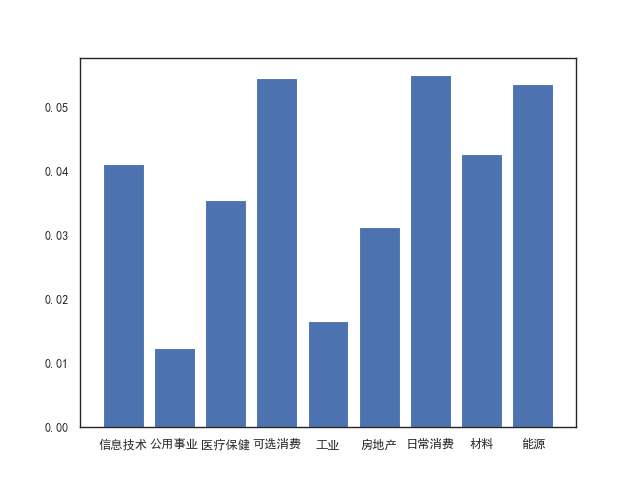
\includegraphics[width=.9\linewidth]{./data/industry.png}
	\caption{\label{fig:industry}违约债分行业分布}
\end{figure}

如表 \ref{fig:industry} 所示,看似较高违约率的行业,
均是因为单一主体违约余额较大(如方正集团导致计算机行业、华晨汽车导致汽车行业、紫光集团导致电子行业、山东如意导致纺织行业违约率激增)。基本可以排除大多数的行业聚类\cite{azizpour2018exploring},即某行业因行业景气集中某段时间违约的情况。即便是近期的房地产违约风波,也并非主要由于行业景气,而是由于房地产“三条红线”等政策约束。因此本文将主要考虑房地产政策(房地产行业且时间大于 2020 年),而不考虑行业本身。

\begin{figure}[htbp]
	\centering
	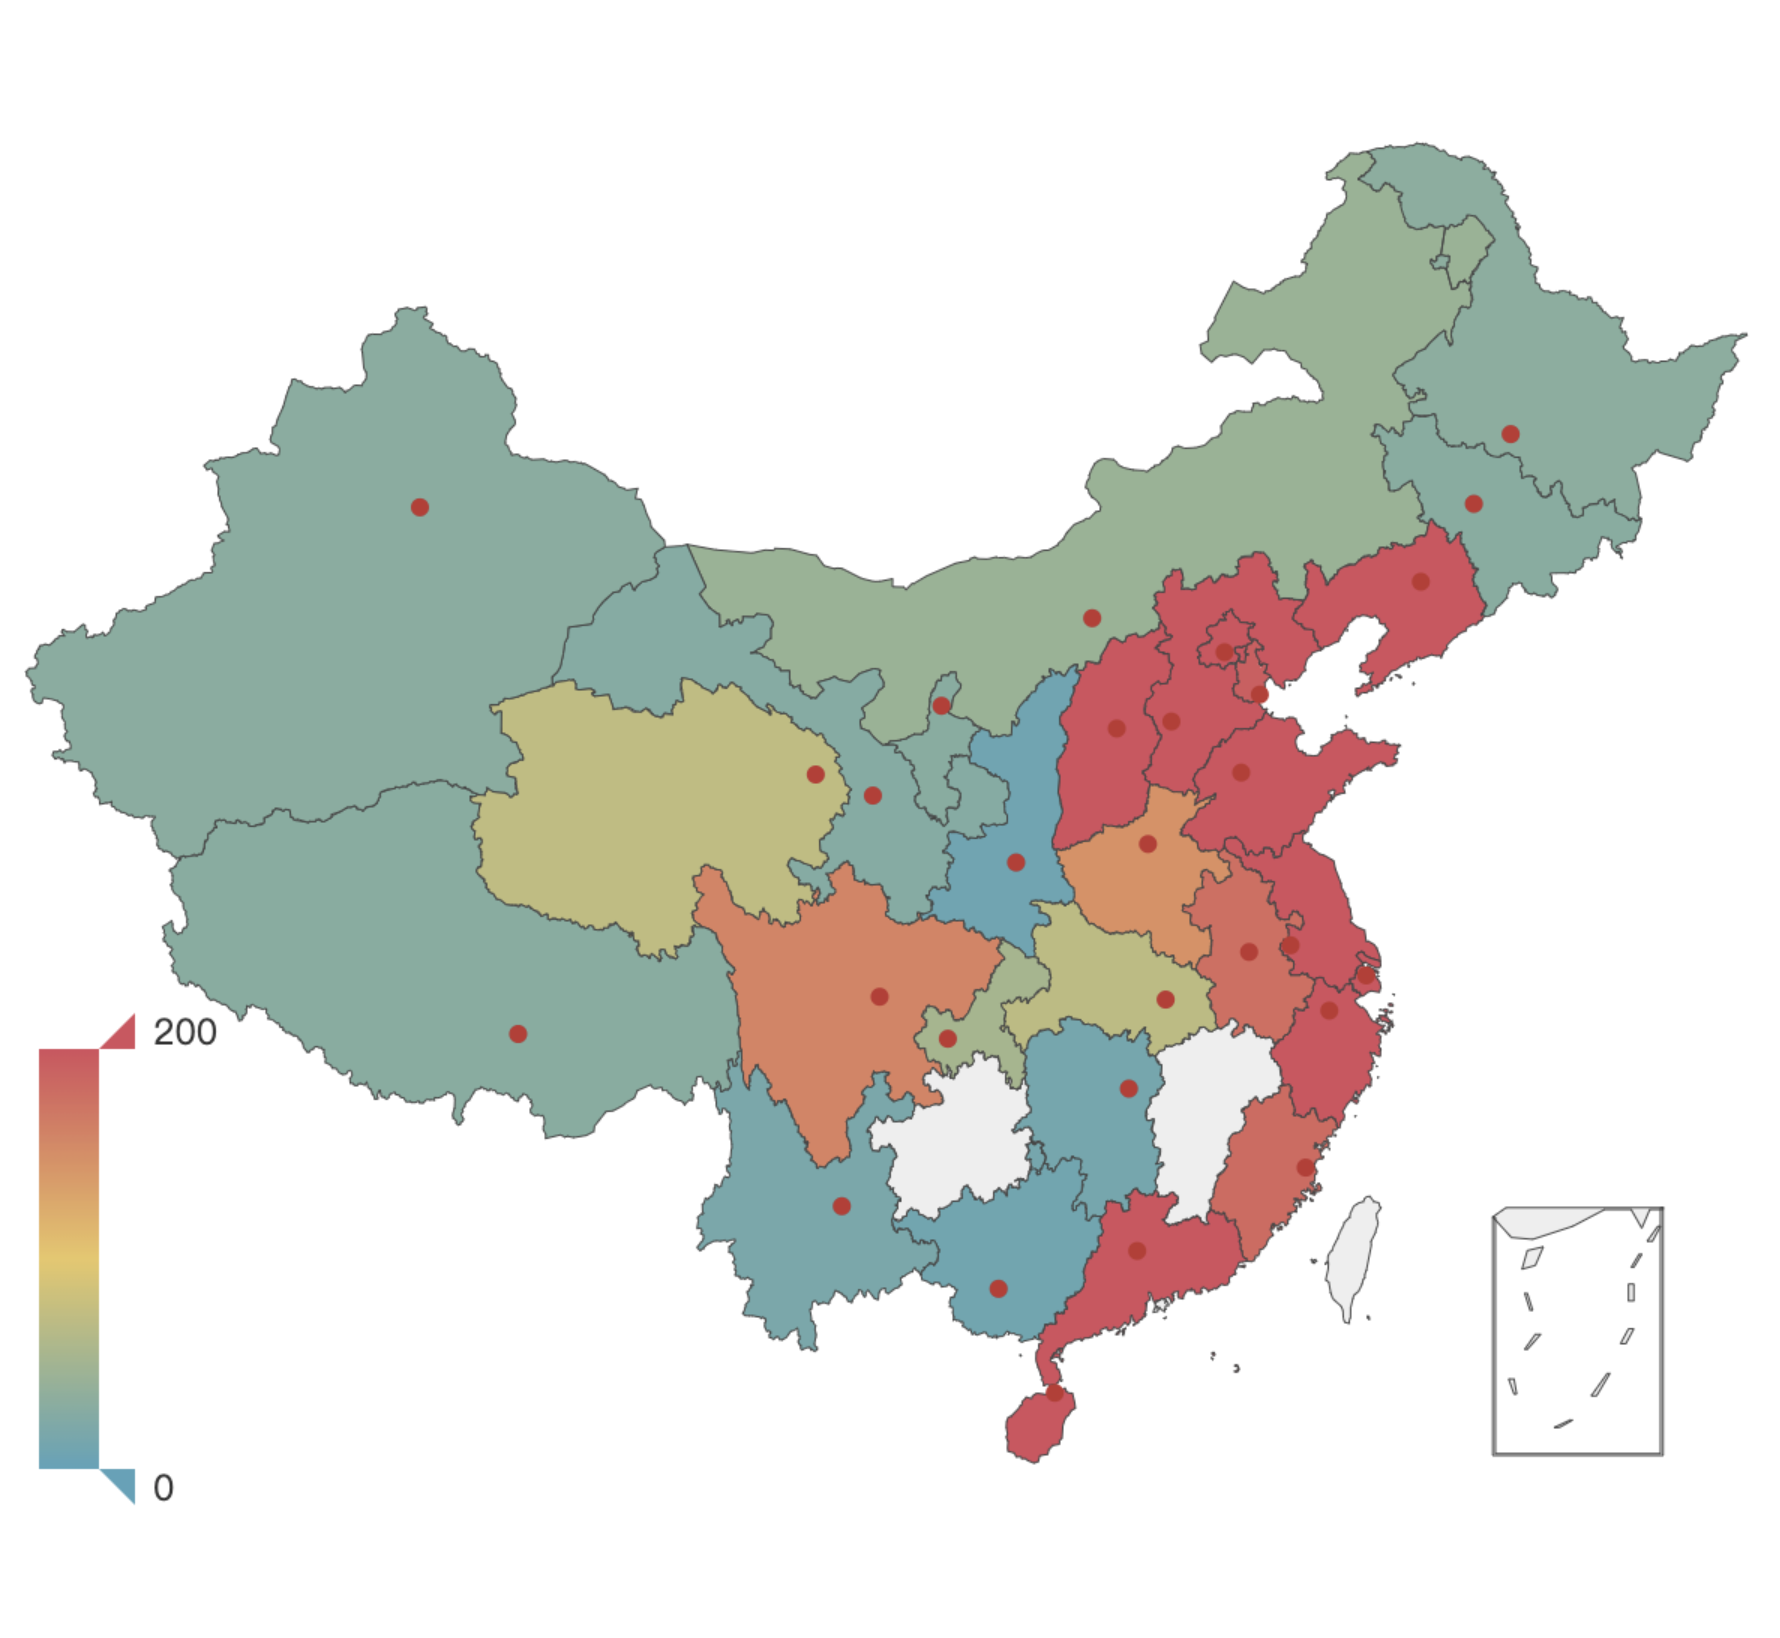
\includegraphics[width=.9\linewidth]{./data/default_by_geo.png}
	\caption{\label{fig:geo}违约债地理分布}
\end{figure}
地理上看,
一方面经济落后地区违约风险较大,一方面经济较好的地区企业发债数量较多可能导致违约金额较大,如图\ref{fig:geo}显示出后一种作用较强。尽管看似部分地区违约率高,但事实上高违约率的原因大多是单一违约主体违约金额大,如河北的华夏幸福、辽宁的华晨宝马、海南的海航、青海的青国投等等。
总的来说地理上的传染尚不明晰,看似地理上的传染更多是因为股权、担保的关系,可能城投债违约后显现出来。

最后是流动性,本文计划以债券成交金额为流动性指标。当市场流动性偏紧时,如永煤违约后各机构连 AAA 国企也不敢买,成交量萎靡流动性偏紧,导致冀中能源、紫光、清华控股等无法发债接续,到期压力巨大,最终部分企业走向违约。
\subsection{宏观层次}
如\ref{sec:zs}中学者研究,货币政策与财政政策可能会对企业违约有影响。本文计划财政政策使用政府支出占GDP比重表征,货币政策以 SHIBOR 利率表征。

有学者对债券回报率做 Fama 因子分析
\cite{chung2019volatility}
,发现以 VIX 指数为代表的波动风险的影响是普遍存在的。
因此本文效仿选择上证 50 期权的隐含波动率作为波动率指标,2015 年期权推出之前则采用上证历史波动率。

\section{计量检验}
\subsection{数据清洗}

我国金融机构和非金融机构之间存在很大的监管差异。金融机构特别是银行、保险等行业在出现风险时,往往由于涉及面众多,可能会引发系统性风险,政府往往会及时采取手段控制风险,如接管安邦保险、明天系的银行、保险等金融机构。因此在建模过程中,我们会在数据中排除掉商业银行、保险公司、证券公司类的金融机构。

城投公司是一个独特的存在。截止 2022 年 2 月,我国信用债券市场中企业债、公司债、中期票据、短融、超短融以及定向工具存量 66.5  万亿,而城投债存量 13 万亿。大多数区县级城投公司以及少数市级城投公司财务状况都很不健康:负债率居高不下,财政回款慢。但迄今为止真正意义上的城投公司违约尚未出现。\Textcite{钟辉勇2016城投债的担保可信吗}指出城投债存在隐性政府背书兜底。例如 2020 年底受永煤信用事件的冲击,投资者对违约的担忧上升、风险偏好下降,出现了“抱团”城投的现象。
2021 年 7 月银保监发 [2021]15 号文指出,各银行保险机构要严格执行地方政府融资相关政策要求,打消财政兜底幻觉,强化合规管理、尽职调查,不得以任何形式新增地方政府隐性债务。或许在将来城投公司违约将逐步正常化,但目前而言城投公司违约的影响因素尚不清晰且与其他企业区别较大,因此我们在数据中亦排除城投债。

最后,我们在回归中加入年份作为控制变量,以控制外生事件冲击,如疫情等。

\subsection{计量回归分析}
如表\ref{tab:logitresult}所示为逻辑斯蒂回归模型结论。

\begin{center}
	\small	\begin{tabular}{p{0.25\linewidth}p{0.2\linewidth}p{0.25\linewidth}p{0.2\linewidth}}
		\hline
		Dep. Variable:   & default          & No. Observations: & 6623       \\
		Model:           & Logit            & Df Residuals:     & 6592       \\
		Method:          & MLE              & Df Model:         & 30         \\
		Date:            & Mon, 14 Feb 2022 & Pseudo R-squ.:    & 0.7014     \\
		Time:            & 13:44:59         & Log-Likelihood:   & -246.83    \\
		converged:       & False            & LL-Null:          & -826.49    \\
		Covariance Type: & nonrobust        & LLR p-value:      & 1.021e-224 \\
	\end{tabular}
	\begin{longtable}{p{0.18\linewidth}p{0.1\linewidth}p{0.1\linewidth}p{0.1\linewidth}p{0.1\linewidth}p{0.12\linewidth}p{0.1\linewidth}}
		\hline
		\textbf{variable}  & \textbf{coef} & \textbf{std err} & \textbf{z} & \textbf{P>|z|} & \textbf{[0.025} & \textbf{0.975]} \\ \hline
		const              & -7.3147       & 2.666            & -2.744     & 0.006          & -12.540         & -2.089          \\ \hline
		评级\_A以上        & -0.1559       & 0.710            & -0.219     & 0.826          & -1.548          & 1.237           \\ \hline
		评级\_B            & 3.1253        & 0.347            & 8.998      & 0.000          & 2.445           & 3.806           \\ \hline
		评级\_C            & 6.7123        & 0.430            & 15.622     & 0.000          & 5.870           & 7.554           \\ \hline
		国有企业           & -3.4180       & 0.733            & -4.660     & 0.000          & -4.856          & -1.980          \\ \hline
		外资企业           & -2.9746       & 0.937            & -3.175     & 0.001          & -4.811          & -1.138          \\ \hline
		民营企业           & -1.7211       & 0.706            & -2.439     & 0.015          & -3.104          & -0.338          \\ \hline
		集体企业           & -2.8521       & 1.117            & -2.554     & 0.011          & -5.041          & -0.663          \\ \hline
		上市企业           & -0.5207       & 0.387            & -1.346     & 0.178          & -1.279          & 0.238           \\ \hline
		持有基金占比       & -0.1531       & 0.135            & -1.131     & 0.258          & -0.418          & 0.112           \\ \hline
		大股东持股比例     & -0.0036       & 0.005            & -0.671     & 0.503          & -0.014          & 0.007           \\ \hline
		主营业务收入(万元) & 5.105e-08     & 2.66e-08         & 1.918      & 0.055          & -1.12e-09       & 1.03e-07        \\ \hline
		应付账款(万元)     & -3.556e-12    & 6.32e-12         & -0.563     & 0.574          & -1.59e-11       & 8.83e-12        \\ \hline
		标准券折算率       & -1.0401       & 1.294            & -0.804     & 0.422          & -3.577          & 1.496           \\ \hline
		净资产(万元)       & -4.853e-08    & 5.58e-08         & -0.871     & 0.384          & -1.58e-07       & 6.07e-08        \\ \hline
		现金短债比         & -0.4579       & 0.406            & -1.129     & 0.259          & -1.253          & 0.337           \\ \hline
		流动性             & -1.482e-10    & 1.58e-10         & -0.938     & 0.348          & -4.58e-10       & 1.61e-10        \\ \hline
		房地产政策         & 2.9309        & 0.977            & 3.000      & 0.003          & 1.016           & 4.845           \\ \hline
		Z                  & -0.0895       & 0.045            & -2.001     & 0.045          & -0.177          & -0.002          \\ \hline
		政府支出/GDP       & 2.0418        & 4.677            & 0.437      & 0.662          & -7.124          & 11.208          \\ \hline
		SHIBOR             & 0.5866        & 0.400            & 1.465      & 0.143          & -0.198          & 1.371           \\ \hline
		波动率             & 0.0671        & 0.033            & 2.002      & 0.045          & 0.001           & 0.133           \\ \hline
		% 发债日\_2014       & 0.0876        & 0.806            & 0.109      & 0.913          & -1.493          & 1.668           \\ \hline
		% 发债日\_2015       & 0.7734        & 0.808            & 0.957      & 0.338          & -0.810          & 2.357           \\ \hline
		% 发债日\_2016       & 2.3629        & 0.945            & 2.502      & 0.012          & 0.512           & 4.214           \\ \hline
		% 发债日\_2017       & 2.1768        & 0.891            & 2.443      & 0.015          & 0.431           & 3.923           \\ \hline
		% 发债日\_2018       & 2.3469        & 0.726            & 3.233      & 0.001          & 0.924           & 3.770           \\ \hline
		% 发债日\_2019       & 2.4301        & 0.928            & 2.618      & 0.009          & 0.610           & 4.250           \\ \hline
		% 发债日\_2020       & 2.5645        & 1.091            & 2.351      & 0.019          & 0.427           & 4.702           \\ \hline
		% 发债日\_2021       & 0.1101        & 1.247            & 0.088      & 0.930          & -2.335          & 2.555           \\ \hline
		% 发债日\_2022       & -15.2080      & 2480.879         & -0.006     & 0.995          & -4877.642       & 4847.226        \\ \hline
		\caption{Logit 模型回归结果}
		\label{tab:logitresult}
	\end{longtable}
\end{center}

微观角度,评级 B/C 的企业,相较于评级 A以上企业违约率明显增加,而 AAA 企业相较于 AA 或 A 违约率差异不大,这是和预期相符的:A 评级及以上企业违约应是预期外事件,评级较低的企业更容易违约。但利用违约前一个月的评级则评级不显著,侧面说明了我国评级用来预测的准确率较低,很多都是在违约即将发生时匆忙调至垃圾级。
国企、外企、集体企业、民营企业违约可能性依次增加亦符合预期:国企可能存在一定的政府支持\autocite{mo2021china},跨国企业通常资金雄厚。
上市公司违约率较低但显著程度不高。
违约本质上还是财务中可用的资金无法覆盖到期应付的债务,因此经营和财务指标对违约的解释力较强。主营收入的增多可以显著冲抵潜在违约的可能性。财务指标 Z 值预警亦显著。

中观角度,房地产政策显著性很高。2020 年以来地产行业受到的冲击较大,企业融资受到约束,之前的高杠杆高周转的无序扩张的苦果使得地产债于 2021 年爆发了违约大潮,几乎所有的违约地产企业都是在 2021 年特别是后半年违约的。

宏观政策对违约显著性不高。我国宏观政策对违约,更多是以稳为主的逆周期调节。因此绝大多数属逆周期的宏观政策对违约的解释力较低。
我国政策更多认为部分企业的违约是一种正常现象,但不希望大规模的集中违约,影响实体经济。如定义地产债危机是“少数企业”的激进扩张导致的,但 2021 年 12 月超预期降准释放流动性,且房贷政策有所放松,以应对恒大的倒下。
但是波动率显著,侧面显示出经济以稳为主的重要性:稳定的经济可以降低违约事件的发生。

在本文的写作过程中,渤海租赁股份有限公司发行的 19 渤海租赁 SCP002 无法兑付本金发生违约,模型预测其接近民企违约率 3\% 处,比较符合预期。
\begin{figure}[h]
	\centering
	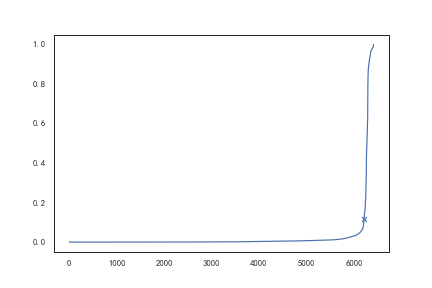
\includegraphics[width=0.9\linewidth]{./data/渤海银行.png}
	\caption{标记处为渤海银行预测点}
	\label{fig:bhyh}
\end{figure}

\subsection{机器学习验证与比较}
违约实际上并非线性的因素叠加,包含了非线性的因素,如华夏幸福违约,既存在过度扩张导致现金流承压,又存在重要股东拒绝为其扩张买单,最终资金链断裂。机器学习适合于提取其中非线性因素。但违约样本是偏态分布的,违约债只占约 1\%,通过神经网络等方式的机器学习会使机器判断有误。综合考虑下决定采用决策树和随机森林两种受样本分布偏态影响较小的方式进行预测。决策树训练结果可视化如图\ref{fig:decision_tree}所示,logit 模型和两种机器学习算法模型准确率如表\ref{tab:acc}所示。


\begin{figure}
	\centering
	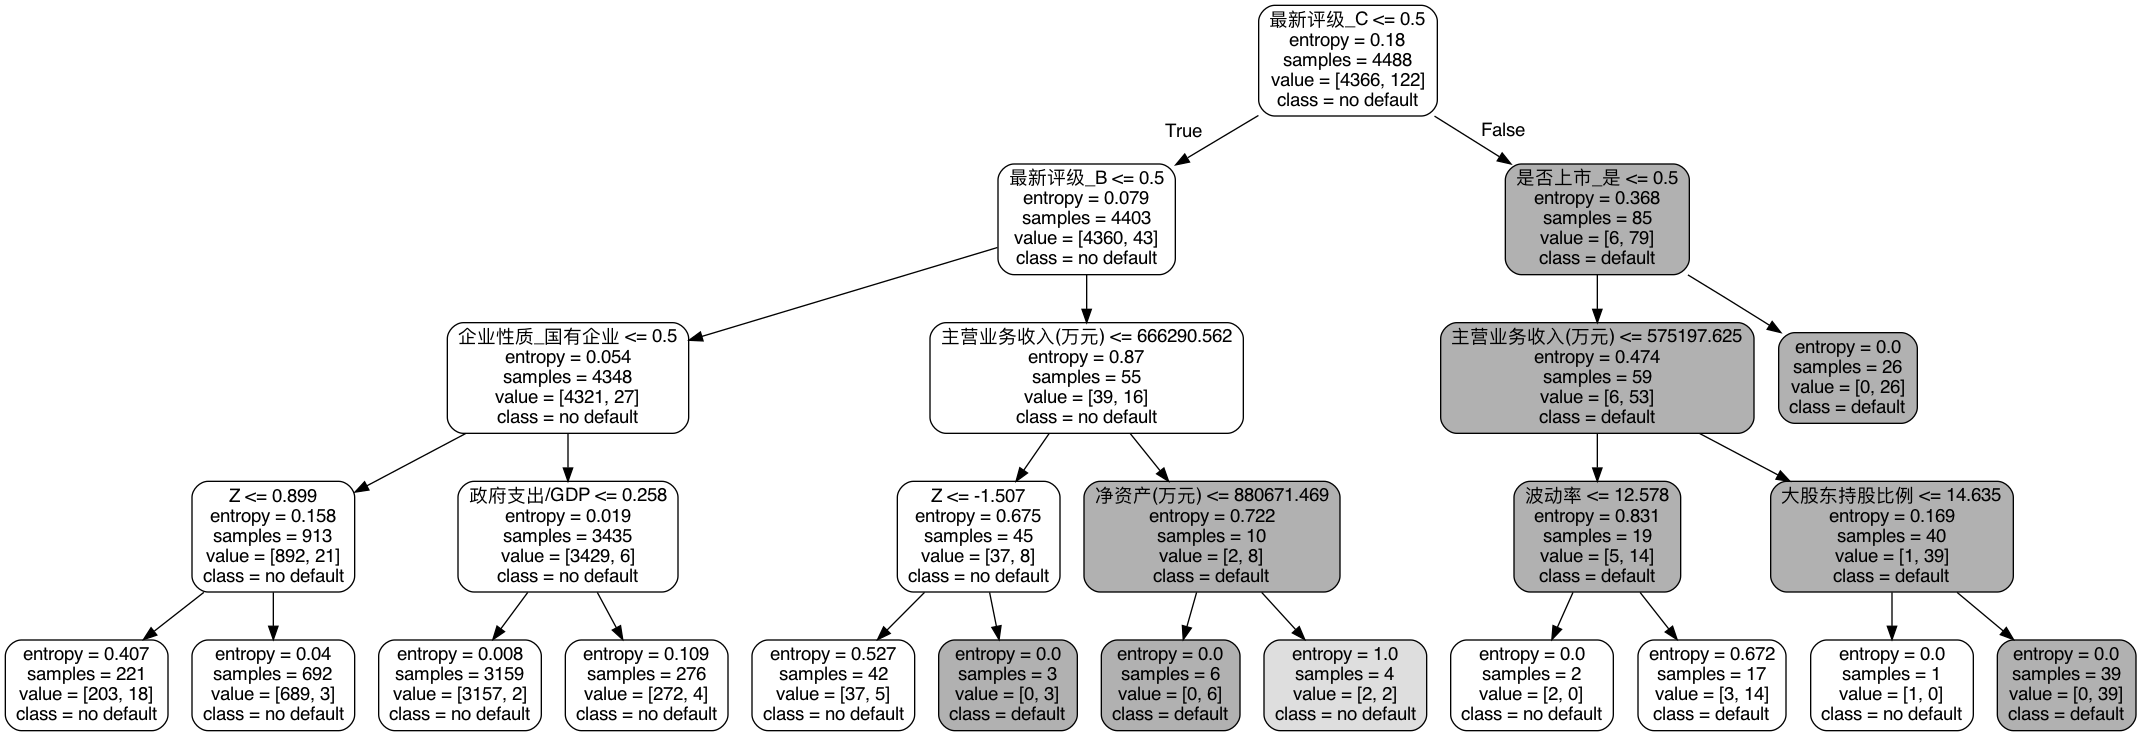
\includegraphics[width=.9\linewidth]{./data/decision_tree.png}
	\caption{\label{fig:decision_tree}决策树}
\end{figure}

图\ref{fig:decision_tree}决策树算法的关键节点如波动率、主营收入、企业性质、Z 值等在 logit 模型中显著,不显著的大股东持股比例分枝后判断的数值仅勉强超过阈值,与 logit 模型互相印证。

\begin{table}
	\caption{\label{tab:acc}不同模型的比较}
	\centering
	\begin{tabular}{lrrrrr}
		                      & accuracy & error rate & precision & recall & f1   \\
		\hline
		全部预测不违约        & 0.99     & 0.01       & -         & 0      & -    \\
		Logistic(全样本)      & 0.99     & 0.01       & 0.86      & 0.72   & 0.78 \\
		Decision Tree(测试集) & 0.99     & 0.01       & 0.93      & 0.73   & 0.82 \\
		Random Forest(测试集) & 0.99     & 0.01       & 0.85      & 0.70   & 0.76 \\
	\end{tabular}
\end{table}

表\ref{tab:acc}中准确率 accuracy 为预测正确的概率,精确率 precision 为预测违约的样本中确实违约的概率,召回率 recall 为事实违约样本中预测正确的概率。精确率和召回率是两个不同方面的机器学习分类器评价指标,其调和平均 F1 > 0.5 则说明分类器是有效的。表\ref{tab:acc}中准确率与全部预测不违约的 0.99 相同,这是由于样本分布偏态造成的。但 F1 值均高于 0.5 ,证明分类器是有效的。且决策树算法显著优于其他算法。

决策树优于 logit 模型算法在于其包含了非线形因素。
而随机森林可能存在一定的训练集上的过拟合。
如图\ref{fig:roc}所示,ROC 曲线的含义是设定任意阈值,得到的真阳性率和假阳性率。随后不断更改阈值,得到 ROC 曲线。AUC 定义为 ROC 曲线下的阈值,AUC面积越大一般认为模型拟合越好。可以看出在训练集上随机森林模型可能存在一定的过拟合,导致 AUC 达到 0.99 ,而 logit 模型在训练集上表现不佳。
\begin{figure}[htbp]
	\centering
	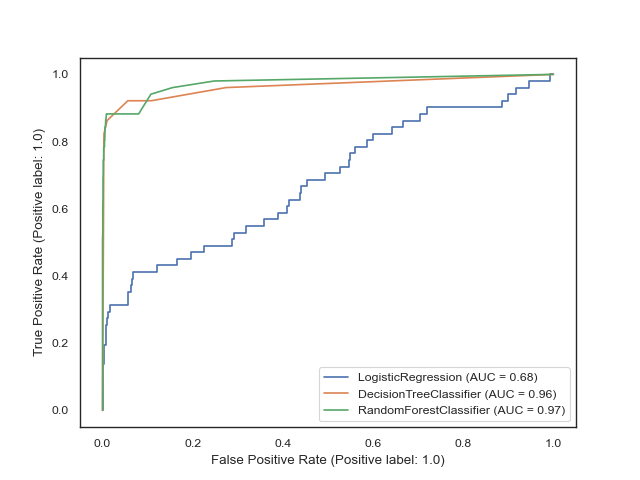
\includegraphics[width=.9\linewidth]{./data/roc.png}
	\caption{\label{fig:roc}ROC曲线与AUC值}
\end{figure}

\section{稳健性检验}
表 \ref{tab:logitresult} 中作为财务指标的 Z 值显著。wind 数据库会直接提供 Z 值给投资者使用,其 Z 值的计算公式为
\begin{equation}
	\label{eq:1}
	Z=1.2X_1+1.4X_2+3.3X_3+0.6X_4+0.999X_5
\end{equation}

式 \ref{eq:1} 中的 \(X_{5}\) 包括了营业收入/总资产,和主营业务收入回归元存在一定的相关性。可能模型中主营业务收入非常显著,因而导致 Z 值显著,而非 Z 值本身带有一定的经济学逻辑。为检验此种可能性,本文将计算 Z 值的元素展开。如果该可能性成立,去掉主营业务收入的情况下,则回归结果 \(\forall i\in [1,2,3,4] X_i\) 应不显著,而仅仅是 \(X_5\) 显著。

\(X_1\)代表营运资本/总资产,\(X_2\)代表留存收益/总资产,\(X_3\)代表息税前利润/总资产:以上变量及 \(X_5\) 均可以直接获得统一的结果;\(X_4\)代表总市值/负债总计,而当企业非上市,总市值数据不可得时,用股东权益代替。

\begin{longtable}{p{0.18\linewidth}p{0.1\linewidth}p{0.1\linewidth}p{0.1\linewidth}p{0.1\linewidth}p{0.12\linewidth}p{0.1\linewidth}}
	\hline
	\textbf{variable} & \textbf{coef} & \textbf{std err} & \textbf{z} & \textbf{P>|z|} & \textbf{[0.025} & \textbf{0.975]} \\ \hline
	\hline
	const             & -3.8725       & 1.252            & -3.092     & 0.002          & -6.327          & -1.418          \\ \hline
	评级\_A以上       & -0.0382       & 0.318            & -0.120     & 0.904          & -0.661          & 0.585           \\ \hline
	评级\_B           & 1.4849        & 0.187            & 7.938      & 0.000          & 1.118           & 1.852           \\ \hline
	评级\_C           & 3.6740        & 0.228            & 16.102     & 0.000          & 3.227           & 4.121           \\ \hline
	国有企业          & -1.6422       & 0.398            & -4.128     & 0.000          & -2.422          & -0.862          \\ \hline
	外资企业          & -1.1744       & 0.467            & -2.514     & 0.012          & -2.090          & -0.259          \\ \hline
	民营企业          & -0.7078       & 0.385            & -1.839     & 0.066          & -1.462          & 0.046           \\ \hline
	集体企业          & -1.2313       & 0.534            & -2.307     & 0.021          & -2.277          & -0.185          \\ \hline
	上市企业          & -0.1945       & 0.192            & -1.014     & 0.310          & -0.570          & 0.181           \\ \hline
	持有基金占比      & -0.0783       & 0.080            & -0.973     & 0.331          & -0.236          & 0.079           \\ \hline
	大股东持股比例    & -0.0013       & 0.003            & -0.508     & 0.611          & -0.006          & 0.004           \\ \hline
	应付账款(万元)    & 1.409e-12     & 2.48e-12         & 0.567      & 0.570          & -3.46e-12       & 6.28e-12        \\ \hline
	标准券折算率      & -0.3647       & 0.651            & -0.560     & 0.575          & -1.640          & 0.911           \\ \hline
	净资产(万元)      & 9.314e-09     & 1.1e-08          & 0.847      & 0.397          & -1.22e-08       & 3.09e-08        \\ \hline
	现金短债比        & -0.1082       & 0.133            & -0.816     & 0.415          & -0.368          & 0.152           \\ \hline
	流动性            & -5.276e-11    & 6.63e-11         & -0.796     & 0.426          & -1.83e-10       & 7.72e-11        \\ \hline
	政府支出/GDP      & 1.2248        & 2.087            & 0.587      & 0.557          & -2.866          & 5.315           \\ \hline
	SHIBOR            & 0.3573        & 0.190            & 1.881      & 0.060          & -0.015          & 0.730           \\ \hline
	波动率            & 0.0341        & 0.016            & 2.135      & 0.033          & 0.003           & 0.065           \\ \hline
	房地产政策        & 0.7415        & 0.411            & 1.805      & 0.071          & -0.064          & 1.547           \\ \hline
	X1                & -0.0083       & 0.003            & -3.009     & 0.003          & -0.014          & -0.003          \\ \hline
	X2                & -0.0037       & 0.002            & -2.375     & 0.018          & -0.007          & -0.001          \\ \hline
	X3                & -0.0062       & 0.004            & -1.638     & 0.101          & -0.014          & 0.001           \\ \hline
	X4                & -0.0064       & 0.002            & -3.917     & 0.000          & -0.010          & -0.003          \\ \hline
	X5                & 0.0005        & 0.001            & 0.530      & 0.596          & -0.001          & 0.002           \\ \hline
	\caption{稳健性检验结果}
	\label{tab:robust}
\end{longtable}

回归结果如表 \ref{tab:robust} 所示,与表 \ref{tab:logitresult} 相比基本一致,仅 SHIBOR 利率变为显著,且\(X_1\) 至 \(X_4\) 均显著,说明 Z 值作为一个综合性的财务指标具有一定的预测能力,而非只是受到主营收入的影响导致显著,假设不成立。
